\mysection{Background Information}

\mysubsection{The StreamIt Language}

TODO

%%     StreamIt is a programming language specifically tailored to DSP
%% streaming applications. The user creates a graph composed of four
%% types of StreamIt constructs: \textit{filters},
%% \textit{pipelines}, \textit{splitjoins}, and \textit{feedback
%% loops}. Filters encapsulate the computation done within an
%% application - they represent the blocks mentioned in the previous
%% section. Each filter operates on a one-dimensional `tape' of
%% values (of any type, including structures and arrays).  The other
%% three constructs dictate the type of connections possible between
%% filters. Every construct explicitly states its input type and
%% output type, and can be passed parameters as would be to a
%% procedure.

%%     StreamIt uses a buffer between every pair of filters to
%% hold values. When the input buffer of a construct (equivalent to
%% the output buffer of the previous construct) is appropriately
%% filled, the construct can execute. Execution involves three steps:
%% reading and removing items from the input buffer (consumption);
%% performing computations; putting items in the output buffer
%% (production). We will not consider the intricacies of managing
%% these buffers, and instead refer to the more abstract notion of a
%% tape.

%%     A filter has pre-defined \textit{peek}, \textit{pop}, and
%% \textit{push} rates (StreamIt code examples are given below).
%% During each execution, the filter accesses a maximum of peek
%% values from its input tape, consumes exactly pop input values from
%% its input tape, and produces exactly push values onto its output
%% tape. Since the removal of an input value is technically an access
%% of that input, the peek rate of a filter must be greater than or
%% equal to the pop rate of that filter. The push or pop rate can be
%% zero - the former corresponds to a filter that consumes items but
%% does not produce them (typically the last filter in a sequence)
%% and the latter corresponds to a filter that produces items but
%% does not consume them (typically the first filter in a sequence).
%% All the accesses, outputs, and removals, as well as all the
%% computation is done inside the main body of the filter, known as
%% the work function.

%% \begin{figure}[bthp]
%%   \centering
%%   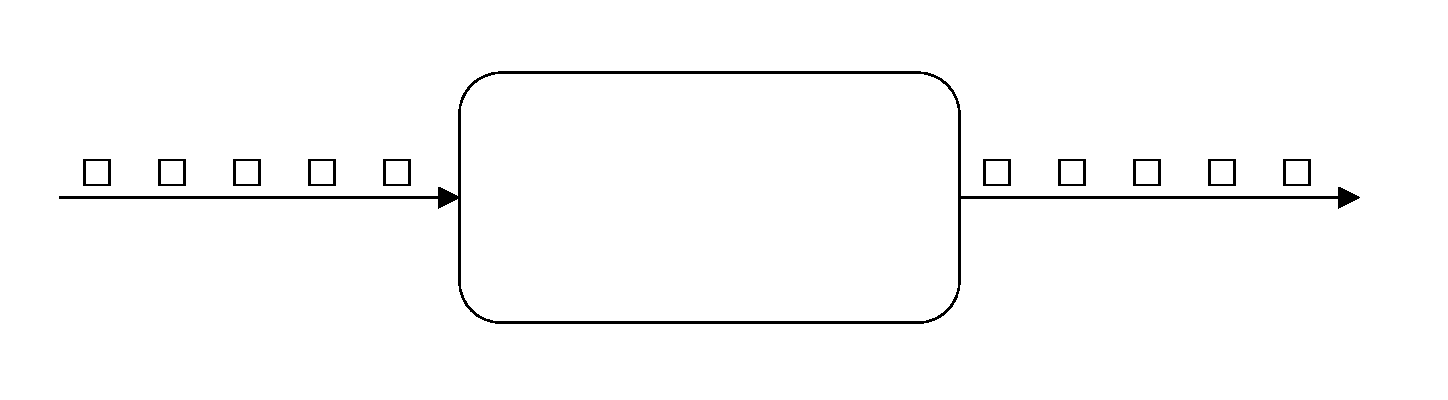
\includegraphics[width=3.0in]{figures/filter.eps}
%%   \caption{StreamIt filter}
%%   \label{fig:filter}
%% \end{figure}

%%     StreamIt also supports a \textit{prework} function, which has its own push,
%% pop, and peek rates.  The prework function executes in place of
%% the work function for the first computation sequence, and is never
%% run again. Additionally, there is an \textit{init} function which
%% is run only once upon creation of the filter, and is usually used
%% to initialize variables.  The init and prework functions are both
%% optional.

%%         A filter can store two types of variables - \textit{field} and
%% \textit{local}. Field variables are declared outside of the
%% specific functions (work, prework, init), and can be accessed from
%% anywhere within the filter. Local variables are declared within a
%% specific function, and only have scope within that function. For
%% example, a variable declared within the init function is local,
%% and could not be accessed within the work function. Therefore, the
%% init function is used to initialize field variables.

%% Code examples of StreamIt filters are shown below.

%% \begin{scriptsize}
%% \begin{singlespace}
%% \begin{verbatim}
%% // This filter adds the parameter scalar to each input.
%% // It does not have an init or prework function
%% float -> float filter scalarAdd(float scalar) {
%%   work push 1 pop 1 peek 1 {
%%     push(scalar + pop());
%%   }
%% }
%% \end{verbatim}
%% \end{singlespace}
%% \end{scriptsize}

%% \begin{scriptsize}
%% \begin{singlespace}
%% \begin{verbatim}
%% // This filter outputs a running average of every three consecutive inputs.
%% // The first time it runs, it ouputs the average of the first two inputs without removing anything from the tape.
%% // It does not have an init function.
%% float -> float filter threeWayAverage() {
%%   prework push 1 pop 0 peek 2 {
%%     float temp;  // example of a local variable
%%     temp = (peek(0)+peek(1))/2;
%%     push(temp);
%%   }
%%   work push 1 pop 1 peek 3 {
%%     float temp;  // example of a local variable
%%     temp = (peek(0) + peek(1) + peek(2))/3
%%     push(temp);
%%     pop()
%%   }
%% }
%% \end{verbatim}
%% \end{singlespace}
%% \end{scriptsize}

%% \begin{scriptsize}
%% \begin{singlespace}
%% \begin{verbatim}
%% // This filter computes an infinite impulse response function.
%% // It does not have a prework function.
%% float->float filter IIR() {
%%     float curr;  // example of a field variable
%%     init {
%%       curr = 0;
%%     }
%%     work push 1 pop 1 peek 3 {
%%       float temp;  \\ example of a local variable
%%       temp = (peek(0) + peek(1) + peek(2))/6;
%%       curr = temp + curr/2;
%%       push(curr);
%%       pop();
%%     }
%% }
%% \end{verbatim}
%% \end{singlespace}
%% \end{scriptsize}

%%     Pipelines, splitjoins, and feedback loops are higher level
%% constructs created from filters. Each structures the layout of its
%% filters in a certain format. Even though these three constructs do
%% not directly provide the syntax to perform computations and work
%% from an input or output tape, they can be thought of as filters in
%% the following way: the construct recieves inputs which are passed
%% to one or more of the filters; all the filters perform
%% computations and pass values to one another through their input
%% and output tapes; the construct outputs values from one or more of
%% its filters. In fact, for every pipeline, splitjoin, and feedback
%% loop there is an equivalent filter representation. Therefore,
%% these three constructs are not strictly necessary for writing a
%% StreamIt program. However, they simplify and structure writing a
%% large application.

%%     The higher level constructs are not limited to combine filters -
%% they can also combine each other. This follows directly from the
%% fact that a higher level construct has some equivalent filter.
%% Therefore, if a pipeline can be composed of filters, it can also
%% be composed of pipelines, splitjoins, and feedback loops, which
%% are all like filters. We shall refer to all four StreamIt
%% constructs generically as blocks. This corresponds to the fact
%% that any StreamIt construct behaves as a block: it takes inputs,
%% performs calculations, and produces outputs.

%%     Pipelines combine a set of blocks in sequential fashion, so that
%% the output of the first block is the input to the second block,
%% the output of the second block is the input to the third block,
%% etc. The blocks are placed in order using the add statement.

%% \begin{figure}[bthp]
%%   \centering
%%   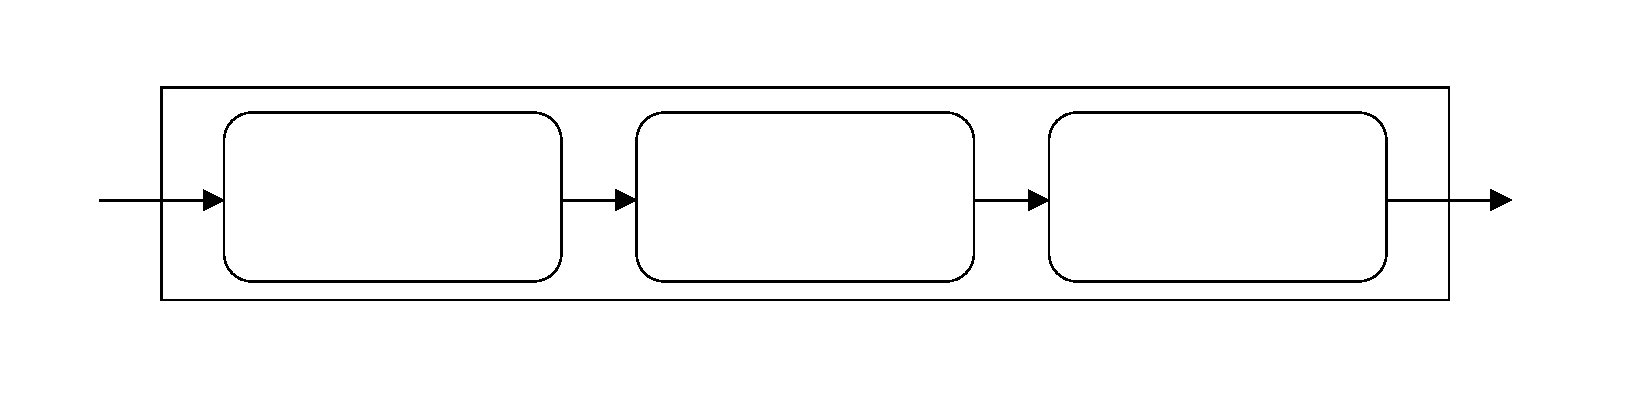
\includegraphics[width=3.0in]{figures/pipeline.eps}
%%   \caption{StreamIt pipeline}
%%   \label{fig:pipeline}
%% \end{figure}

%% \begin{scriptsize}
%% \begin{singlespace}
%% \begin{verbatim}
%% // This pipeline connects the filters scalarAdd and threeWayAverage.
%% // The parameter scalar passed to this pipeline is passed to the
%% // filter scalarAdd.
%% float -> float pipeline combinedWork(float scalar) {
%%   add scalarAdd(scalar);
%%   add threeWayAverage();
%% }
%% \end{verbatim}
%% \end{singlespace}
%% \end{scriptsize}

%%     A splitjoin arranges blocks in a parallel fashion.  The inputs to
%% a splitjoin are sent to each block in a \textit{roundrobin} or
%% \textit{duplicate} manner, and the outputs of each block are
%% joined in a roundrobin manner. Duplicate splitting means the
%% inputs to the splitjoin are copied and sent to each block, so that
%% each block receives exactly the same set of inputs.  Roundrobin
%% splitting means the inputs to the splitjoin are sent to each block
%% according to user defined weights.  For example, the first block
%% receives two inputs, the second block receives one input, the
%% third block receives two inputs.  Therefore, each block sees a
%% different set of inputs. Roundrobin joining (the only type of
%% joining permitted) means the outputs of each block are combined
%% according to user defined weights, and these represent the outputs
%% of the entire splitjoin. Blocks are listed in the order which they
%% recieve inputs using add statements. The way inputs are sent is
%% determined by using the split statement before the block list, and
%% the way outputs are recieved is determined by using the join
%% statement after the block list.

%% \begin{figure}[bthp]
%%   \centering
%%   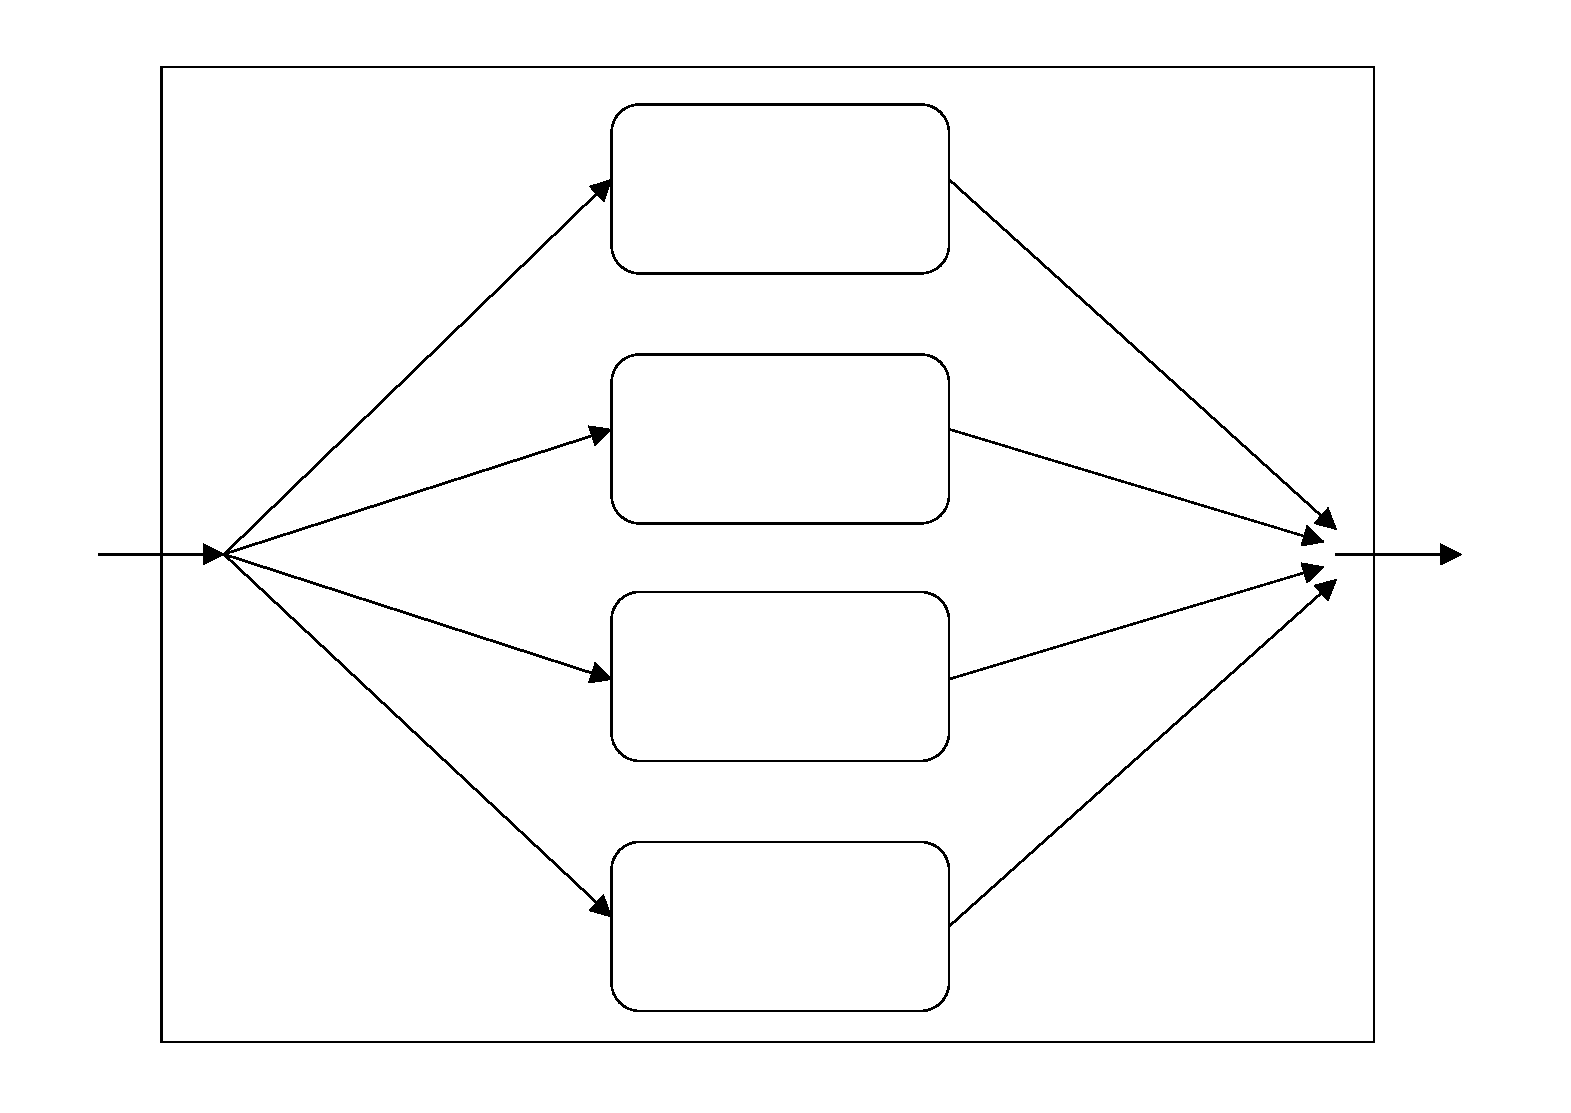
\includegraphics[width=3.0in]{figures/splitjoin.eps}
%%   \caption{StreamIt splitjoin}
%%   \label{fig:splitjoin}
%% \end{figure}

%% \begin{scriptsize}
%% \begin{singlespace}
%% \begin{verbatim}
%% // This splitjoin splits its inputs three ways.
%% // The first two inputs are sent to the first block, the next
%% // input to the second block, and the next two inputs to the third
%% // block.
%% // The outputs are collected in the following manner: three from
%% //the first block, five from the second block, and four from the
%% // third block.
%% // For every 2+1+2=5 values inputted, 3+5+4=12 values are
%% // outputted.
%% float -> float splitjoin mySplitjoin() {
%%  split roundrobin(2,1,2);
%%   add combinedWork(3.5);
%%   add combinedWork(4.5);
%%   add threeWayAverage();
%% join roundrobin(3,5,4);
%% }
%% \end{verbatim}
%% \end{singlespace}
%% \end{scriptsize}

%%     A feedback loop uses some of its output as
%% an input. It consists of a body block and a loop block. The input
%% to the entire feedback loop is combined with the output of the
%% loop block and sent to the body block, via a roundrobin joiner.
%% The output of the body block is split two ways in a roundrobin or
%% duplicate manner.  The first set of outputs is used as the output
%% of the entire feedback loop, and the second set of outputs is used
%% as the input to the loop block. Note that there must be initial
%% values enqueued on the output tape of the loop block in order for
%% the feedback loop to begin executing. The first statement in a
%% feedback loop is a join, determining how inputs are sent to the
%% body block. The body and loop blocks are listed next. The last
%% statement is a split, determining where outputs are sent from the
%% loop block.

%% \begin{figure}[bthp]
%%   \centering
%%   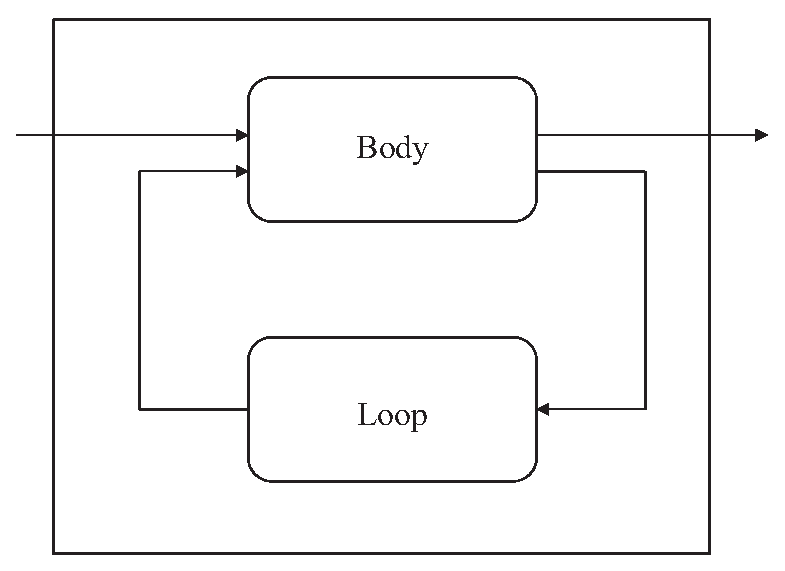
\includegraphics[width=3.0in]{figures/feedback.eps}
%%   \caption{StreamIt feedback loop}
%%   \label{fig:feedback}
%% \end{figure}

%% \begin{scriptsize}
%% \begin{singlespace}
%% \begin{verbatim}
%% // This is a feedback loop implementation of the IIR filter.
%% // The body and loop are both anonymous filters.
%% float -> float feedbackloop IIRFeedback() {
%%   join roundrobin(3,1);
%%   body float->float filter {
%%     work push 1 pop 1 peek 4 {
%%       push((peek(0)+peek(1)+peek(2))/6 + peek(3)/2);
%%       pop();
%%     }
%%   };
%%   loop float->float filter {
%%     work push 1 pop 1 peek 1 {
%%       push(pop());
%%     }
%%   };
%%   split duplicate();
%%   enqueue(0.0);
%% }
%% \end{verbatim}
%% \end{singlespace}
%% \end{scriptsize}

%%     To run a program, the StreamIt compiler finds a
%% steady-state schedule of the number of times to execute each
%% filter \cite{Karczmarek}. If such a schedule cannot be found, the
%% user created block diagram is ill-formed and could not represent a
%% real world application.

%% \mysubsection{Block Representations}

%%     The execution of a block (StreamIt or otherwise) can by
%% characterized by a single equation if the block is linear, and a
%% pair of equations if the block is state-space linear. We describe
%% these terms in detail below.

%% \mysubsubsection{Linear Representations}

%%     A block is termed linear if its outputs are a linear
%% combination of its inputs plus a set of constants. In mathematical
%% terms, this relationship can be modelled by the equation
%% $\vec{\mathbf{y}} = \mathbf{D}\vec{\mathbf{u}} +
%% \vec{\mathbf{b}}$, where $\vec{\mathbf{u}}$ is a column vector
%% representing the inputs, $\mathbf{D}$ is a matrix representing the
%% weights applied to each input, $\vec{\mathbf{b}}$ is a column
%% vector representing constants added to the inputs, and
%% $\vec{\mathbf{y}}$ is a column vector representing the outputs.

%%     Suppose we have the following linear model:
%% \starteqnstar
%% \vec{\mathbf{y}} = \left [ \begin{array} {cc} 1 & 2 \\ 3 & 4 \\
%% 5 & 6 \end{array} \right ] \vec{\mathbf{u}} + \left [
%% \begin{array} {c} 7
%% \\ 8 \\ 9 \end{array}\right ]
%% \doneeqnstar

%%     It is exactly described by the following StreamIt filter:
%% \begin{scriptsize}
%% \begin{singlespace}
%% \begin{verbatim}
%% int -> int filter linearFilter() {
%%   work push 3 pop 2 peek 2 {
%%     push(1*peek(0) + 2*peek(1) + 7);
%%     push(3*peek(0) + 4*peek(1) + 8);
%%     push(5*peek(0) + 6*peek(1) + 9);
%%     pop(); pop();
%%   }
%% }
%% \end{verbatim}
%% \end{singlespace}
%% \end{scriptsize}

%%     A process for analyzing and optimizing linear StreamIt filters
%% is described in \cite{Lamb}.

\mysubsection{State-Space Representations}

    A general way of representing a block is by a state-space model.
A set of variables captures the `state' of the filter, so that the
output is a combination of these variables (termed state
variables) and the inputs. Additionally, the states themselves
change upon every execution of the block. This is represented by
the two equations:
\starteqnstar
\vspace{-12pt}
\vec{\mathbf{y}} & = & g(\vec{\mathbf{x}},\vec{\mathbf{u}}) \\
\vec{\dot{\mathbf{x}}} & = & f(\vec{\mathbf{x}},\vec{\mathbf{u}})
\doneeqnstar

    The state vector is denoted by $\vec{\mathbf{x}}$, the inputs by $\vec{\mathbf{u}}$,
and the outputs by $\vec{\mathbf{y}}$. $\vec{\dot{\mathbf{x}}}$
represents the new state vector, i.e. the state vector after it is
updated. The first equation is for the outputs, the second
equation is for the state updates.

    A linear state-space model has the additional property that
the state updates and outputs are linear in the state variables
and inputs. We can use a simpler set of equations:
\starteqnstar
\vec{\mathbf{y}} & = & \mathbf{C}\vec{\mathbf{x}}  +
\mathbf{D}\vec{\mathbf{u}} \\
\vec{\dot{\mathbf{x}}} & = & \mathbf{A}\vec{\mathbf{x}} +
\mathbf{B}\vec{\mathbf{u}}
\doneeqnstar

    $\mathbf{A}$, $\mathbf{B}$, $\mathbf{C}$, and $\mathbf{D}$ are
matrices whose dimensions depend on the number of states, inputs,
and outputs. Not all blocks can be represented by a linear
state-space model. However, a linear state-space model is more
general than a linear model, so a wider class of blocks can be
represented. We will not discuss general state-space models any
further in this paper, therefore we will write state-space instead
of linear state-space for conciseness.

    Suppose we have the following state-space model:
\starteqnstar
\vec{\mathbf{y}} & = & \left [ \begin{array} {cc} 11 & 12
\end{array} \right ] \vec{\mathbf{x}} + \left [ \begin{array} {ccc} 13 & 14 & 15 \end{array} \right
 ] \vec{\mathbf{u}} \\
\vec{\dot{\mathbf{x}}} & = & \left [ \begin{array} {cc} 1 & 2 \\ 6
& 7 \end{array} \right ] \vec{\mathbf{x}} + \left [ \begin{array} {ccc} 3 & 4 & 5 \\
8 & 9 & 10 \end{array} \right ] \vec{\mathbf{u}}
\doneeqnstar

    It is exactly described by the following StreamIt filter:
\begin{singlespace}
\vspace{-12pt}
\begin{scriptsize}
\begin{verbatim}
    int -> int filter stateSpaceFilter() {
      int x1, x2;
      work push 1 pop 3 peek 3 {
        int x1_temp, x2_temp;
        push(11*x1 + 12*x2 + 13*peek(0) + 14*peek(1) + 15*peek(2));
        x1_temp = 1*x1 + 2*x2 + 3*peek(0) + 4*peek(1) + 5*peek(2);
        x2_temp = 6*x1 + 7*x2 + 8*peek(0) + 9*peek(1) + 10*peek(2);
        x1 = x1_temp;
        x2 = x2_temp;
        pop(); pop(); pop();
      }
    }   
\end{verbatim}
\end{scriptsize}
\vspace{-12pt}
\end{singlespace}

    Note we introduced two extra variables - $x1\_temp$ and $x2\_temp$.
We do this because we do not want to overwrite the old values for
$x1$ and $x2$ until all the new values are calculated. Also, we
have made no provisions for constants as in the linear model. This
issue is resolved in the next section.
